\documentclass[10pt,handout,compress,professionalfont]{beamer}
%\documentclass[10pt,compress,professionalfont]{beamer}



\usepackage[latin1]{inputenc}
\usepackage{graphicx}
%\usepackage{pgf}

\usepackage{pstricks} 
\usepackage{pstricks-add} 
\usepackage{pst-plot} 
\usepackage{pst-text,pst-node,pst-tree} 

\usepackage{beamerthemeAmsterdam} 

%\hypersetup{pdfstartview={FitH}}


\setbeamertemplate{navigation symbols}{}
%\usetheme{Warsaw}
%\usecolortheme{beaver}
%\usefonttheme{structuresmallcapsserif}


\title[Point-Based Color Bleeding With Volumes]{PCBEX:\\Point-Based Color Bleeding With Volumes\\Thesis Defense}
\author{Christopher James Gibson}
\institute{California Polytechnic University\\CSC Department}
\date{June 9, 2011}

\setcounter{tocdepth}{1}

\begin{document}

\AtBeginSection[]
{
  \begin{frame}<beamer>
    \frametitle{Outline}
    \tableofcontents[currentsection,currentsubsection]
  \end{frame}
}




%%----------------------------------------------------------------------  TITLE
\begin{frame}

    \titlepage

\end{frame}




%%-------------------------------------------------------------------  SCHEDULE
\begin{frame}{Schedule}

\tableofcontents

\end{frame}




\section{Introduction}
%%---------------------------------------------------------------  INTRODUCTION
\begin{frame}{Graphics Intro}

    \begin{columns}
        \begin{column}{0.65\textwidth}
            {\bf Rendering} is the process of producing 2D images from a 3D scene description\\
            \vspace{8mm}
            At its core, all of {\bf computer graphics} is the visualization of how light interacts in these scenes\\
            \vspace{8mm}
            Modelling physically correct light interactions can get extremely computationally expensive\\
        \end{column}
        \begin{column}{0.35\textwidth}
                \includegraphics[width=\textwidth]{../img/external/spanish}
        \end{column}
    \end{columns}

\end{frame}




\subsection{Global Illumination}
%%--------------------------------------------  BACKGROUND: GLOBAL ILLIMUNATION
\begin{frame}{Global Illumination}

    \begin{columns}
        \begin{column}{0.65\textwidth}
            {\bf Global Illumination} represents the set of algorithms that estimate complex lighting systems\\
            \vspace{8mm}
            The results lead to richer, more realistic images\\

        \end{column}
        \begin{column}{0.35\textwidth}
            \vspace{-8mm}
            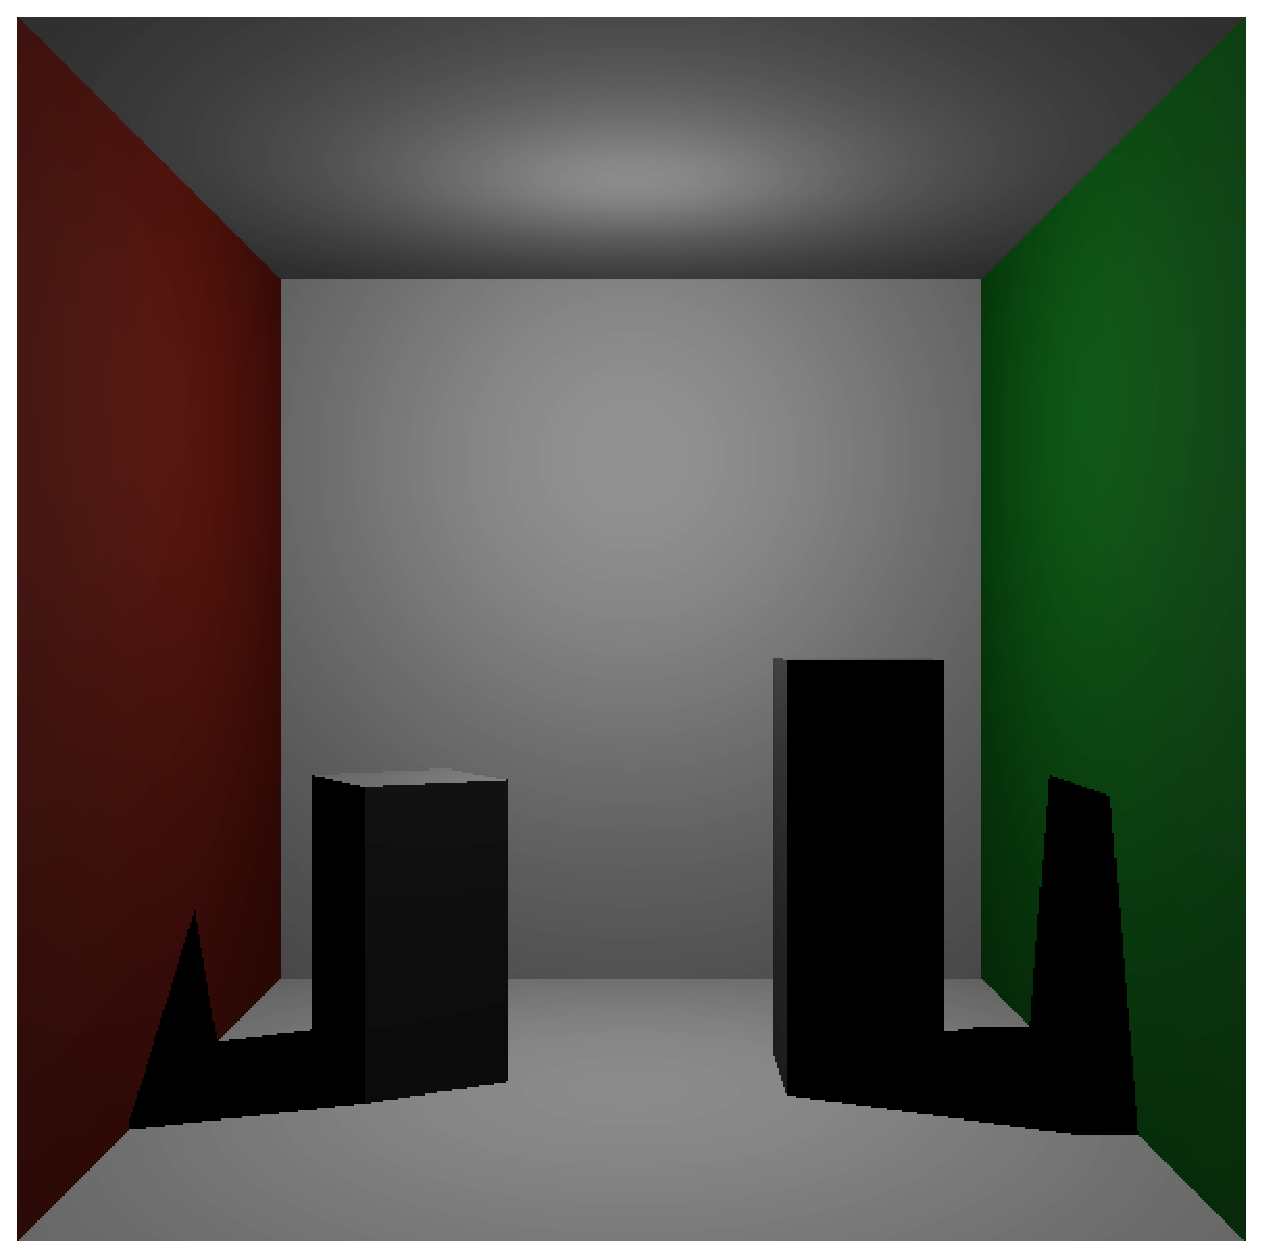
\includegraphics[width=\textwidth]{../img/boxes_noindirect}\\
            {\centering\scriptsize Direct Lighting\\}
            \vspace{2mm}
            \includegraphics[width=\textwidth]{../img/indirect_box_high}\\
            {\centering\scriptsize Direct Lighting \& Global Illumination\\}
        \end{column}
    \end{columns}

\end{frame}




\subsection{Point-Based Color Bleeding}
%%------------------------------------------------  BACKGROUND: VOLUME LIGHTING
\begin{frame}{Point-Based Color Bleeding (PCB)}


    \begin{columns}
        \begin{column}{0.65\textwidth}
            Cheap, accurate global illumination effects using color bleeding\\
            \vspace{8mm}
            Utilizes direct light point cloud representation of scene's direct lighting\\
            \vspace{8mm}
            Already used heavily in production due to its performance advantages

        \end{column}
        \begin{column}{0.35\textwidth}
            \vspace{-4mm}
            \includegraphics[width=\textwidth]{../img/external/pcb}\\
            {\centering\scriptsize Surfels in PCB\\}
        \end{column}
    \end{columns}

\end{frame}




\subsection{Motivation}
%%------------------------------------------  RELATED WORK: GLOBAL ILLIMUNATION
\begin{frame}{Motivation}

    \begin{columns}
        \begin{column}{0.35\textwidth}
            {\centering \includegraphics[width=\textwidth]{../img/bunny_spot_sad}\\}

        \end{column}
        \begin{column}{0.65\textwidth}
            Complex volume lighting algorithms are computationally expensive and complex\\
            \vspace{8mm}
            Most GA algorithms do not include volume contributions\\
            
        \end{column}
    \end{columns}
\end{frame}




\subsection{Goals}
%%------------------------------------------  RELATED WORK: GLOBAL ILLIMUNATION
\begin{frame}{Goals}

    \begin{columns}
        \begin{column}{0.5\textwidth}

            \vspace{-4mm}
            \begin{itemize}
                \item Modify existing PCB in order to include volumetric lighting\\ \vspace{2mm}
                \item Accurately model scatter, absorption and scatter properties\\ \vspace{2mm}
                \item Modify volume integration algorithm to add scatter-in effect\\ \vspace{2mm}
                \item Return comparable results with shorter overall runtimes
            \end{itemize}
        \end{column}
        \begin{column}{0.5\textwidth}
            \includegraphics[width=\textwidth]{../img/bunny_glow}
        \end{column}
    \end{columns}

\end{frame}




\section{Background}
\subsection{Graphics Background}
%%-----------------------------------------------------------------  BACKGROUND
\subsection{Illumination and Light}
%%---------------------------------------------------  BACKGROUND: ILLIMUNATION
\begin{frame}{Flux and Radiance}

    {\bf Flux} is the measure of total light emitted \textit{(Watts)}

    \begin{varblock}{Radiance \& Radiance Invariance}
        \begin{columns}
            \begin{column}{0.5\textwidth}
                    \[
                    \mathit{L} = \frac{\mathit{d^{2}\Phi}}{\mathit{dw\:dA}^\perp} = \frac{\mathit{d^{2}\Phi}}{\mathit{dw\:dA}\textup{cos}\theta}
                    \]
            \end{column}
            \begin{column}{0.5\textwidth}
                    \[
                        L(x \to y) = L(y \to x)
                    \]
            \end{column}
        \end{columns}
    \end{varblock}

    \begin{varblock}{Irradiance}
        \begin{columns}
            \begin{column}{0.5\textwidth}
                    \[
                    E = \frac{d\Phi}{dA}
                    \]
            \end{column}
            \begin{column}{0.5\textwidth}
                    \[
                        \mathit{E} = \int\mathit{L}(\textup{p} \leftarrow w)\textup{cos}\theta dw
                    \]
            \end{column}
        \end{columns}
    \end{varblock}


        % NOTE: Flux density per unit area, per unit solid angle
        % NOTE: dA is the projection of dA on a plane perpendicular to w
        % NOTE: radiance is incoming light power

\end{frame}




%%---------------------------------------------------  BACKGROUND: ILLIMUNATION
\begin{frame}{Irradiance}

    \centering
    \vspace{-1cm}
    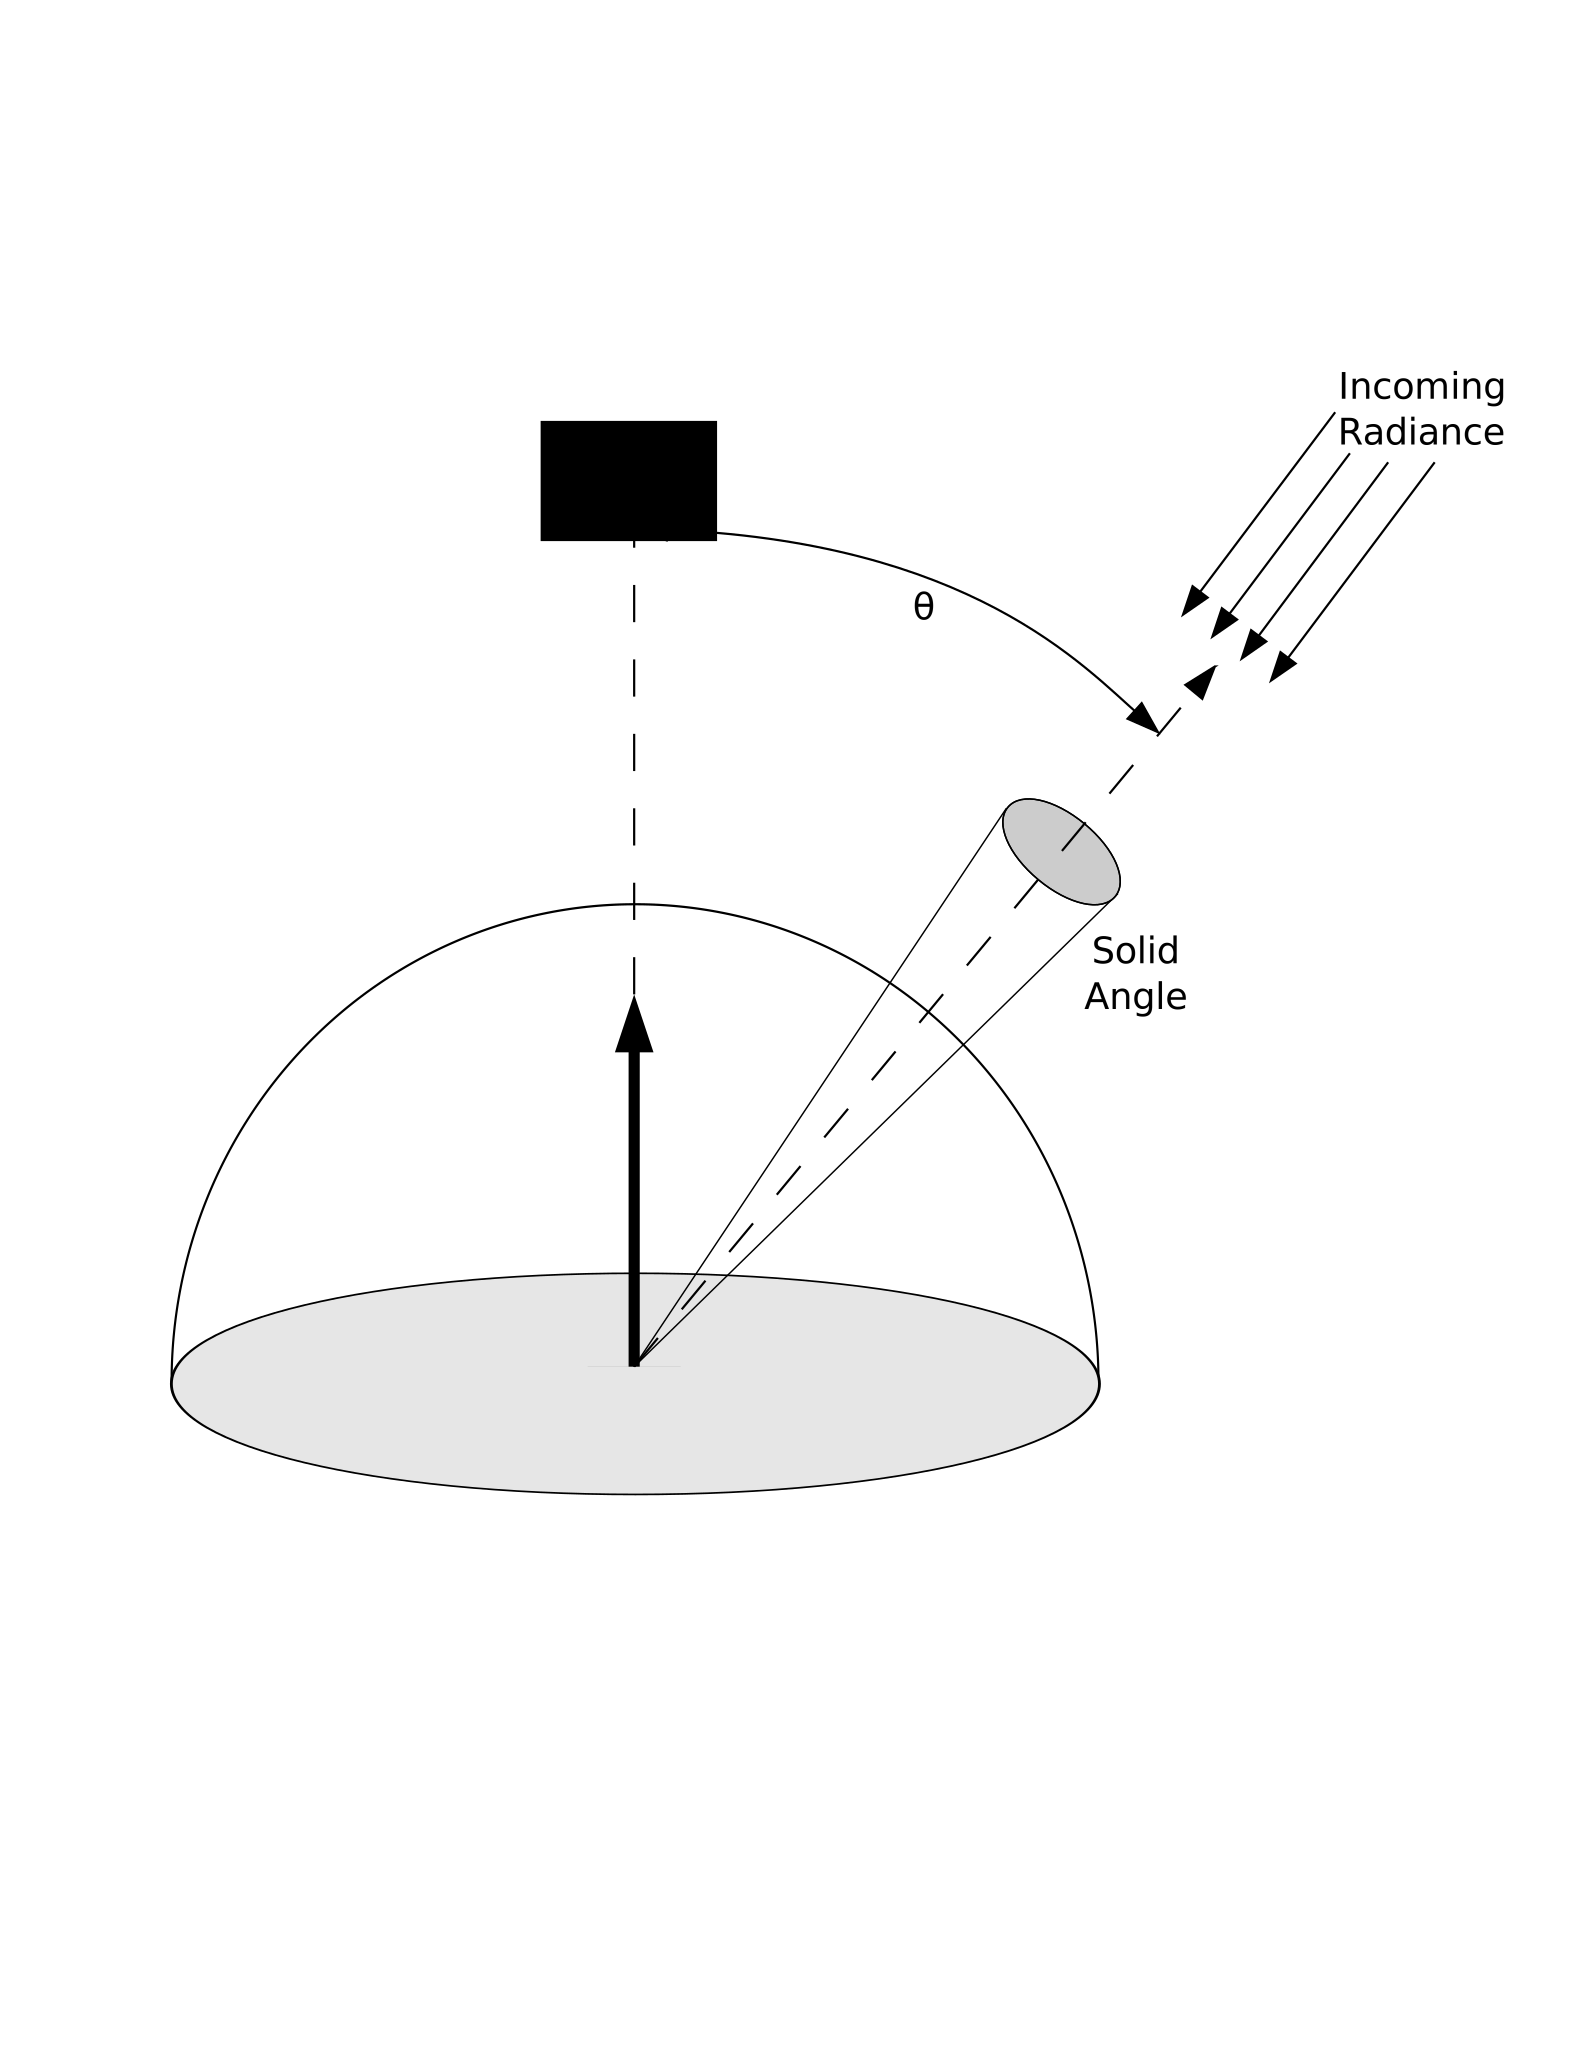
\includegraphics[height=80mm]{../img/diag/radiance.pdf}

\end{frame}




\subsection{BRDF}
%%-----------------------------------------------------------  BACKGROUND: BRDF
\begin{frame}{BRDF and BSRDF}


    \begin{block}{BRDF}
        \begin{center}
            {\bf B}idirectional {\bf R}eflectance {\bf D}istribution {\bf F}unction

            \vspace{3mm}

            Gives us a formalism for describing the reflection from a surface
        \end{center}

        \[
            \mathit{dE}(\textup{p}, w_i) = \int\mathit{L_i}(\textup{p} \leftarrow w_i)\textup{cos}\theta_i dw_i.
        \]
    \end{block}
    
    \begin{block}{BSRDF}
        \begin{center}
            {\bf B}idirectional {\bf S}cattering-surface {\bf R}eflectance {\bf D}istribution {\bf F}unction

            \vspace{3mm}

            Describes complex behavior of light within surface

            (\emph{subsurface scattering}.)
        \end{center}
    \end{block}

\end{frame}



\subsection{Volume Lighting}
%%---------------------------------------------------  BACKGROUND: ILLIMUNATION
\begin{frame}{Volume Lighting}

    \centering
    \vspace{0cm}
    
\includegraphics[width=100mm]{../img/diag/vol_scatter.pdf}

\end{frame}




\subsection{Volume Lighting}
%%---------------------------------------------------  BACKGROUND: ILLIMUNATION
\begin{frame}{Volume Lighting}

    \begin{columns}
        \begin{column}{0.55\textwidth}

            \vspace{-10mm}
            \begin{block}{Absorption}
                \[
                    e^{-\int_{0}^{d}\sigma_{a} (p+t\mathit{w},\mathit{w})d\mathit{t}}
                \]
            \end{block}

            \begin{block}{Scatter Out}
                \[
                    d\mathit{L}_{o}(\textup{p},w) = -\sigma_{s}(\textup{p},w) \mathit{L}_{i}(\textup{p},-w)dt
                \]
            \end{block}

        \end{column}
        \begin{column}{0.45\textwidth}
            \vspace{-4mm}
            \includegraphics[width=\textwidth]{../img/external/scatter}\\
            {\centering\scriptsize Extinction in a volume\\}
        \end{column}
    \end{columns}

\end{frame}




%%---------------------------------------------------  BACKGROUND: ILLIMUNATION
\begin{frame}{Volume Lighting}


    \begin{columns}
        \begin{column}{0.5\textwidth}

            \vspace{-10mm}
            \begin{block}{Phase Function}
                Described as $phase(w \to w')$
            \end{block}

            \begin{block}{Source Normalization}
                \[
                    \int_{\mathbb{S}^2}phase(w \to w')\textup{d}w' = 1.
                \]
            \end{block}

        \end{column}
        \begin{column}{0.5\textwidth}
            \vspace{-4mm}
            \includegraphics[width=\textwidth]{../img/diag/phase_func_sm}\\
            {\centering\scriptsize Phase function distribution\\}
        \end{column}
    \end{columns}

\end{frame}




%%---------------------------------------------------  BACKGROUND: ILLIMUNATION
\begin{frame}{Volume Lighting}

    \begin{block}{Transmittance}
        \[
            T_{r}(\textup{p} \to \textup{p}') = e^{-\int_{0}^{d}\sigma (p+t\mathit{w},\mathit{w})d\mathit{t}}.
        \]
    \end{block}

    \begin{block}{Scatter In}
        \[
            \mathit{S}(\textup{p},w) = \mathit{L}_{\textup{ve}}(\textup{p},w) + \sigma_{\textup{s}}(\textup{p}, w) \int_{\mathbb{S}^2} phase(\textup{p}, -w' \to w) L_{i}(\textup{p},w')\textup{d}w'.
        \]
    \end{block}

\end{frame}




\subsection{Monte Carlo Integration}
%%-----------------------------------------------  BACKGROUND WORK: MONTE CARLO
\begin{frame}{Monte Carlo Integration}


    \begin{columns}
        \begin{column}{0.6\textwidth}

    \vspace{-10mm}
    Monte Carlo methods allow estimation of complex systems through use of probability functions and random numbers.\\
    \vspace{8mm}

    Most useful to us is Monte Carlo Integration.

        \end{column}
        \begin{column}{0.4\textwidth}
            \vspace{-4mm}
            \includegraphics[width=\textwidth]{../img/external/MonteCarloIntegrationCircle}\\
            {\centering\scriptsize Randomly sampling a circle\\}
        \end{column}
    \end{columns}

\end{frame}




\section{Related Work}
\subsection{Global Illumination}
%%------------------------------------------  RELATED WORK: GLOBAL ILLIMUNATION
\begin{frame}{Related Works: Global Illumination}

    Field of study in computer graphics.

    Photon Mapping.

    Radiosity.

    Monte Carlo Techniques.

\end{frame}




%%------------------------------------------  RELATED WORK: GLOBAL ILLIMUNATION
\begin{frame}{Related Works: Point-Based Color Bleeding}



    \begin{columns}
        \begin{column}{0.6\textwidth}

    \vspace{-10mm}
    Point-Based Approximate Color Bleeding by Per Christensen.\\
    \vspace{8mm}

    Subset of scene geometry is thoroughly sampled, creating point cloud.\\
    \vspace{8mm}

    Point cloud is sampled to determin incoming radiance.

        \end{column}
        \begin{column}{0.4\textwidth}
            \vspace{-4mm}
            \includegraphics[width=\textwidth]{../img/pcloud}\\
            {\centering\scriptsize Randomly sampling a circle\\}
        \end{column}
    \end{columns}

\end{frame}




%%------------------------------------------  RELATED WORK: GLOBAL ILLIMUNATION
\begin{frame}{Related Works: Photon Mapping}

    \begin{columns}
        \begin{column}{0.5\textwidth}

    \vspace{-10mm}

    Photons cast from lights interact with the scene.  At each hit, a photon can:
    
    \begin{itemize}
        \item Bounce\\
        \vspace{2mm}

        \item Pass Through\\
        \vspace{2mm}

        \item Be Absorbed\\
    \end{itemize}

        \end{column}
        \begin{column}{0.5\textwidth}
            \vspace{-4mm}
            \includegraphics[width=\textwidth]{../img/external/ewr7_mcbox.jpg}
        \end{column}
    \end{columns}
\end{frame}




\subsection{Volume Rendering}
%%---------------------------------------------  RELATED WORK: VOLUME RENDERING
\begin{frame}{Related Works: Volume Rendering}

    \begin{columns}
        \begin{column}{0.6\textwidth}

    \vspace{-10mm}

    Seminal research involved number of approaches...
    
    \begin{itemize}
        \item Polygonalization of straight voxels \textit{(boxy)}\\
        \vspace{4mm}

        \item Polygonal representation based on isosurfaces\\
        \vspace{4mm}

        \item Opacity/Color arrays \textit{(interpolation across voxels)}\\
    \end{itemize}

        \end{column}
        \begin{column}{0.4\textwidth}
            \vspace{-4mm}
            \includegraphics[width=\textwidth]{../img/external/img188}\\
            {\centering\scriptsize Renders of CT scan data\\}
        \end{column}
    \end{columns}
\end{frame}




%%---------------------------------------------  RELATED WORK: VOLUME RENDERING
\begin{frame}{Related Works: Volume Rendering}

    \begin{columns}
        \begin{column}{0.7\textwidth}

    \vspace{-5mm}
    Multi-resolution volumes help save on memory and allow for on-demand loading\\
    \vspace{8mm}

    Occlusion techniques involving volume acceleration structures help avoid extraneous computations

        \end{column}
        \begin{column}{0.3\textwidth}
            \vspace{-4mm}
            \includegraphics[width=\textwidth]{../img/external/vol_multi_res}\\
            {\centering\scriptsize Renders of CT scan data\\}
        \end{column}
    \end{columns}

\end{frame}




\section{PCB Extension Algorithm}
\subsection{Point-Based Color Bleeding}
%%--------------------------------------------------------------  PCB EXTENSION
\begin{frame}{Point-Based Color Bleeding}

    \begin{enumerate}
        \item Sample the scene and generate a point cloud
        \item Perform ray tracing on regular geometry
        \item Replace ambient estimates with a gather stage using surrounding point cloud
    \end{enumerate}

\end{frame}




\subsection{Extension Overview}
%%--------------------------------------------------------------  PCB EXTENSION
\begin{frame}{Extension Overview}

    \begin{enumerate}
        \item Sample the scene and generate a point cloud
        \item Sample the participating media and evaluate scatter, absorbtion and direct lighting
        \item Cast rays as normal
        \item Orient hemispherical samples along the normals of the surfaces intersected
        \item Model scatter-out and scatter-in properties during lighting gather stage
    \end{enumerate}

\end{frame}




\subsection{Sampling the Scene}
%%--------------------------------------------------------------  PCB EXTENSION
\begin{frame}{Sampling the Scene}

    \begin{columns}
        \begin{column}{0.5\textwidth}

    \vspace{-5mm}
    Rays are cast and intersections with objects are recorded\\
    \vspace{8mm}

    Sampling "camera" is behind normal camera with wider field of view\\
    \vspace{8mm}

    Surfels are oriented at the intersections aligned along the surface normal

        \end{column}
        \begin{column}{0.5\textwidth}
            \vspace{-4mm}
            \includegraphics[width=\textwidth]{../img/diag/surfel_samp_mod.pdf}\\
        \end{column}
    \end{columns}

\end{frame}




\subsection{Gathering Light}
%%--------------------------------------------------------------  PCB EXTENSION
\begin{frame}{Gathering Light}

    \begin{columns}
        \begin{column}{0.5\textwidth}

    \vspace{-5mm}
    At render time, rays are cast from normal camera\\
    \vspace{8mm}

    Samples are cast from intersecting surface oriented along its normal

        \end{column}
        \begin{column}{0.5\textwidth}
            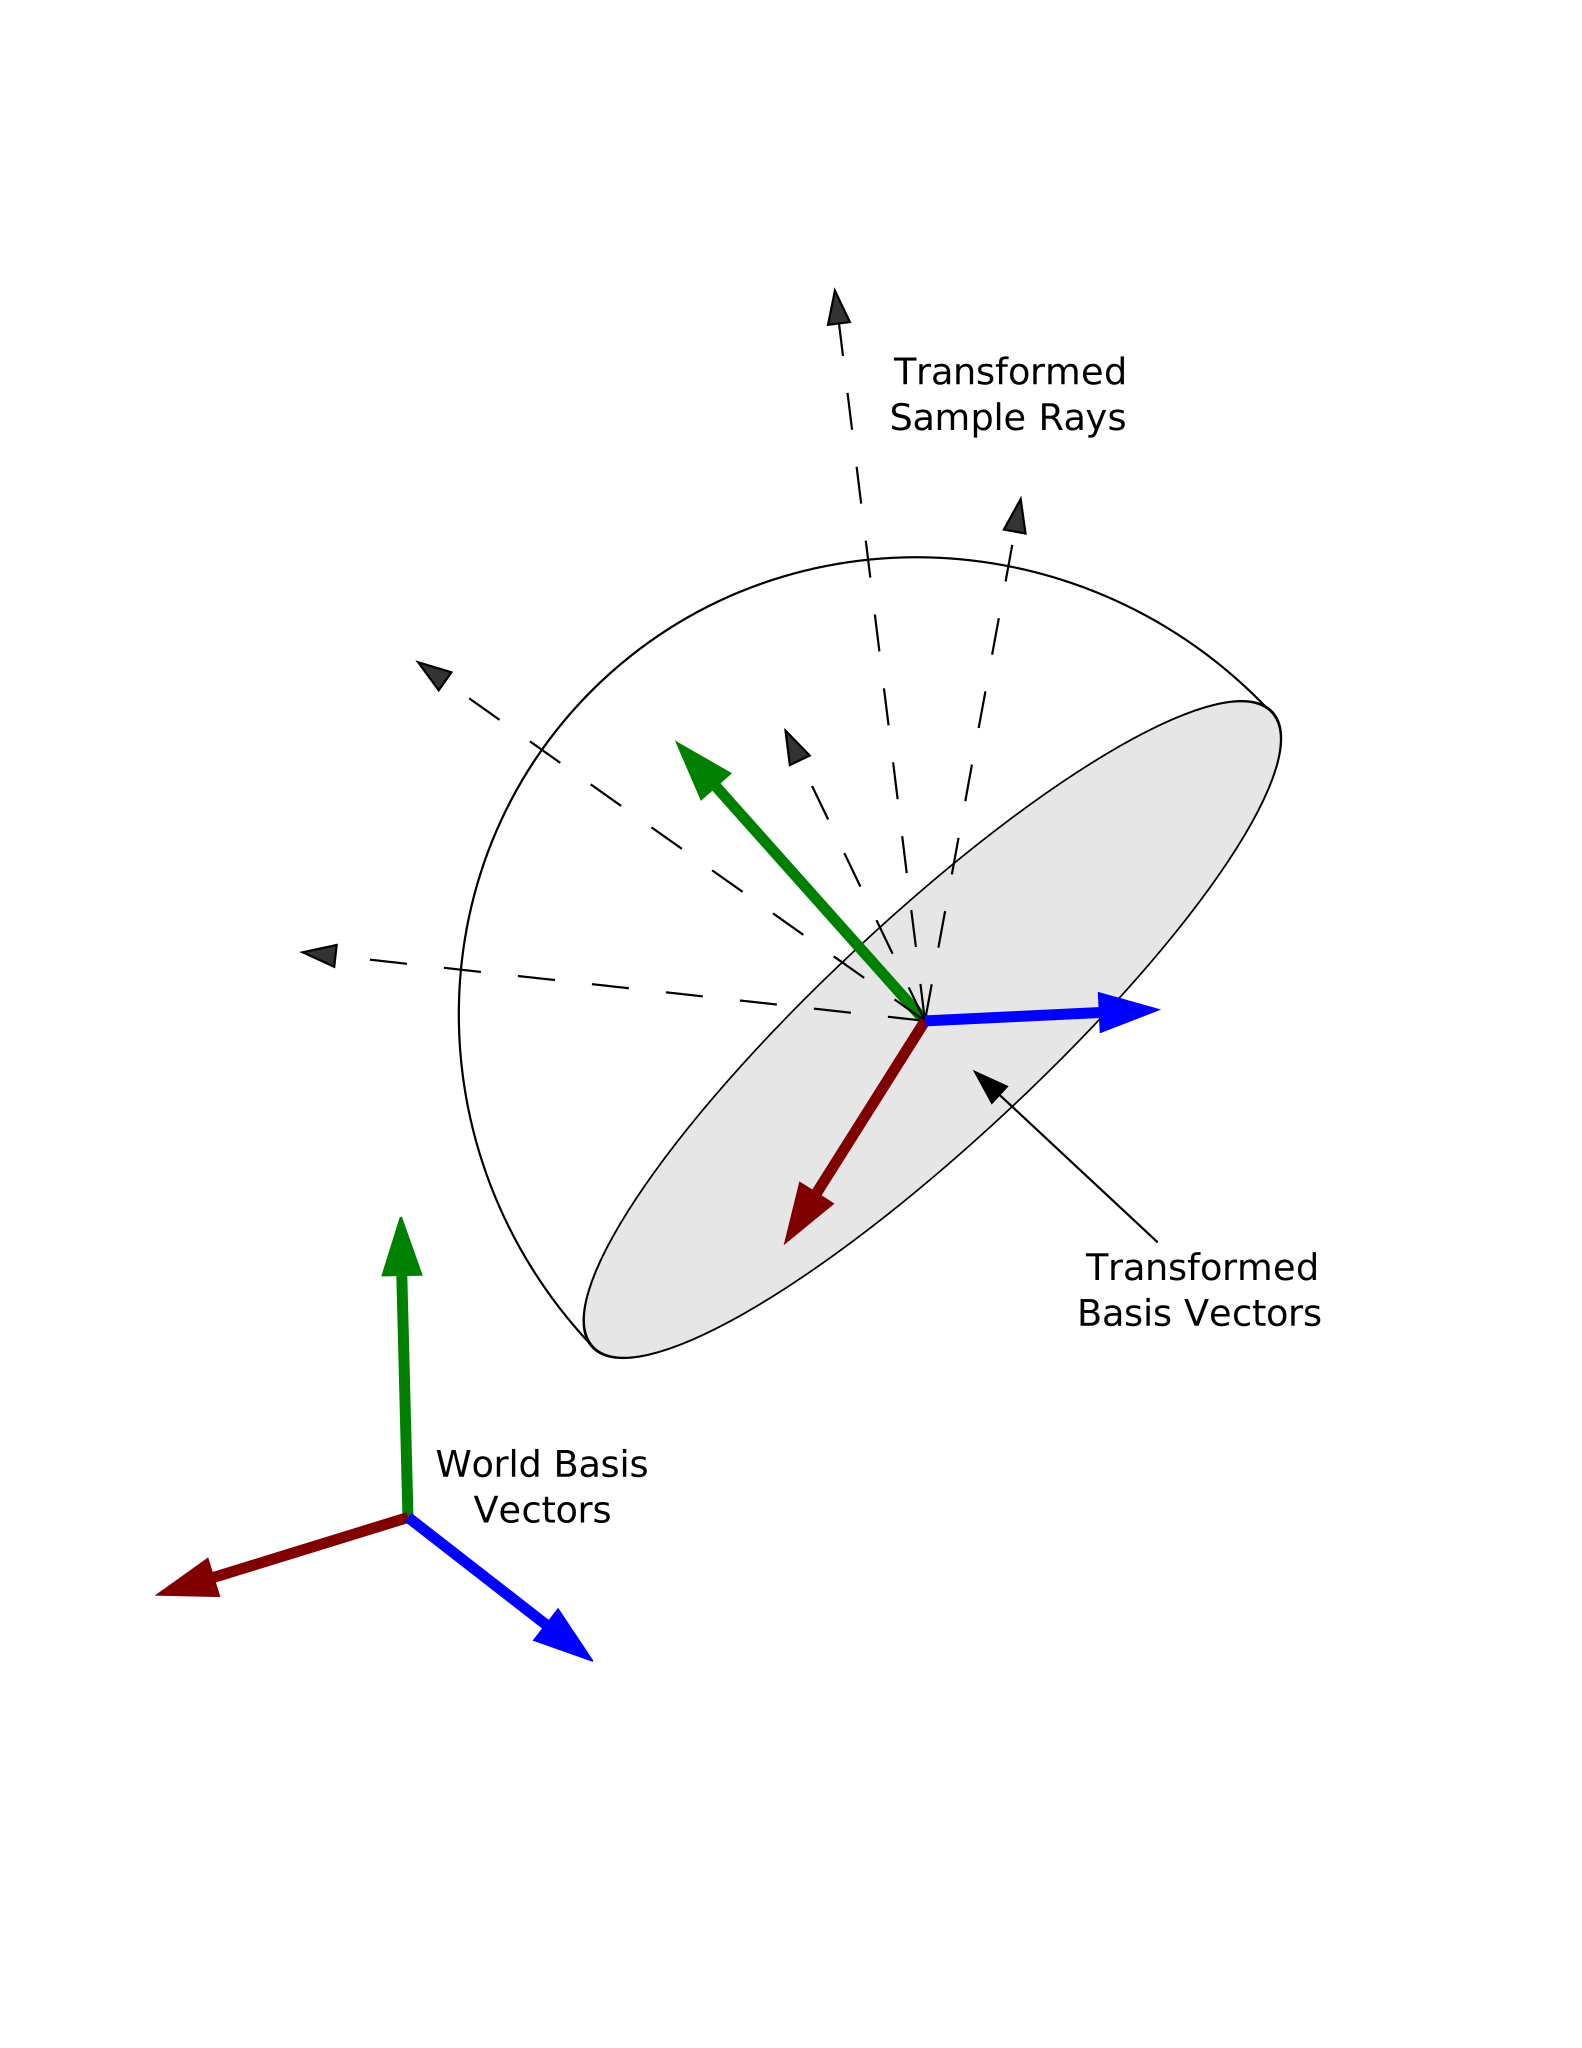
\includegraphics[width=\textwidth]{../img/diag/orthnormal.pdf}\\
            \vspace{-4mm}
        \end{column}
    \end{columns}

\end{frame}




\subsection{Gathering Light}
%%--------------------------------------------------------------  PCB EXTENSION
\begin{frame}{Gathering Light}

    \begin{columns}
        \begin{column}{0.5\textwidth}

    \vspace{-5mm}
    Samples cast into point cloud "gather" light via intersection\\
    \vspace{8mm}

    Samples are returned and used to evaluate the integral over the aligned hemisphere

        \end{column}
        \begin{column}{0.5\textwidth}
            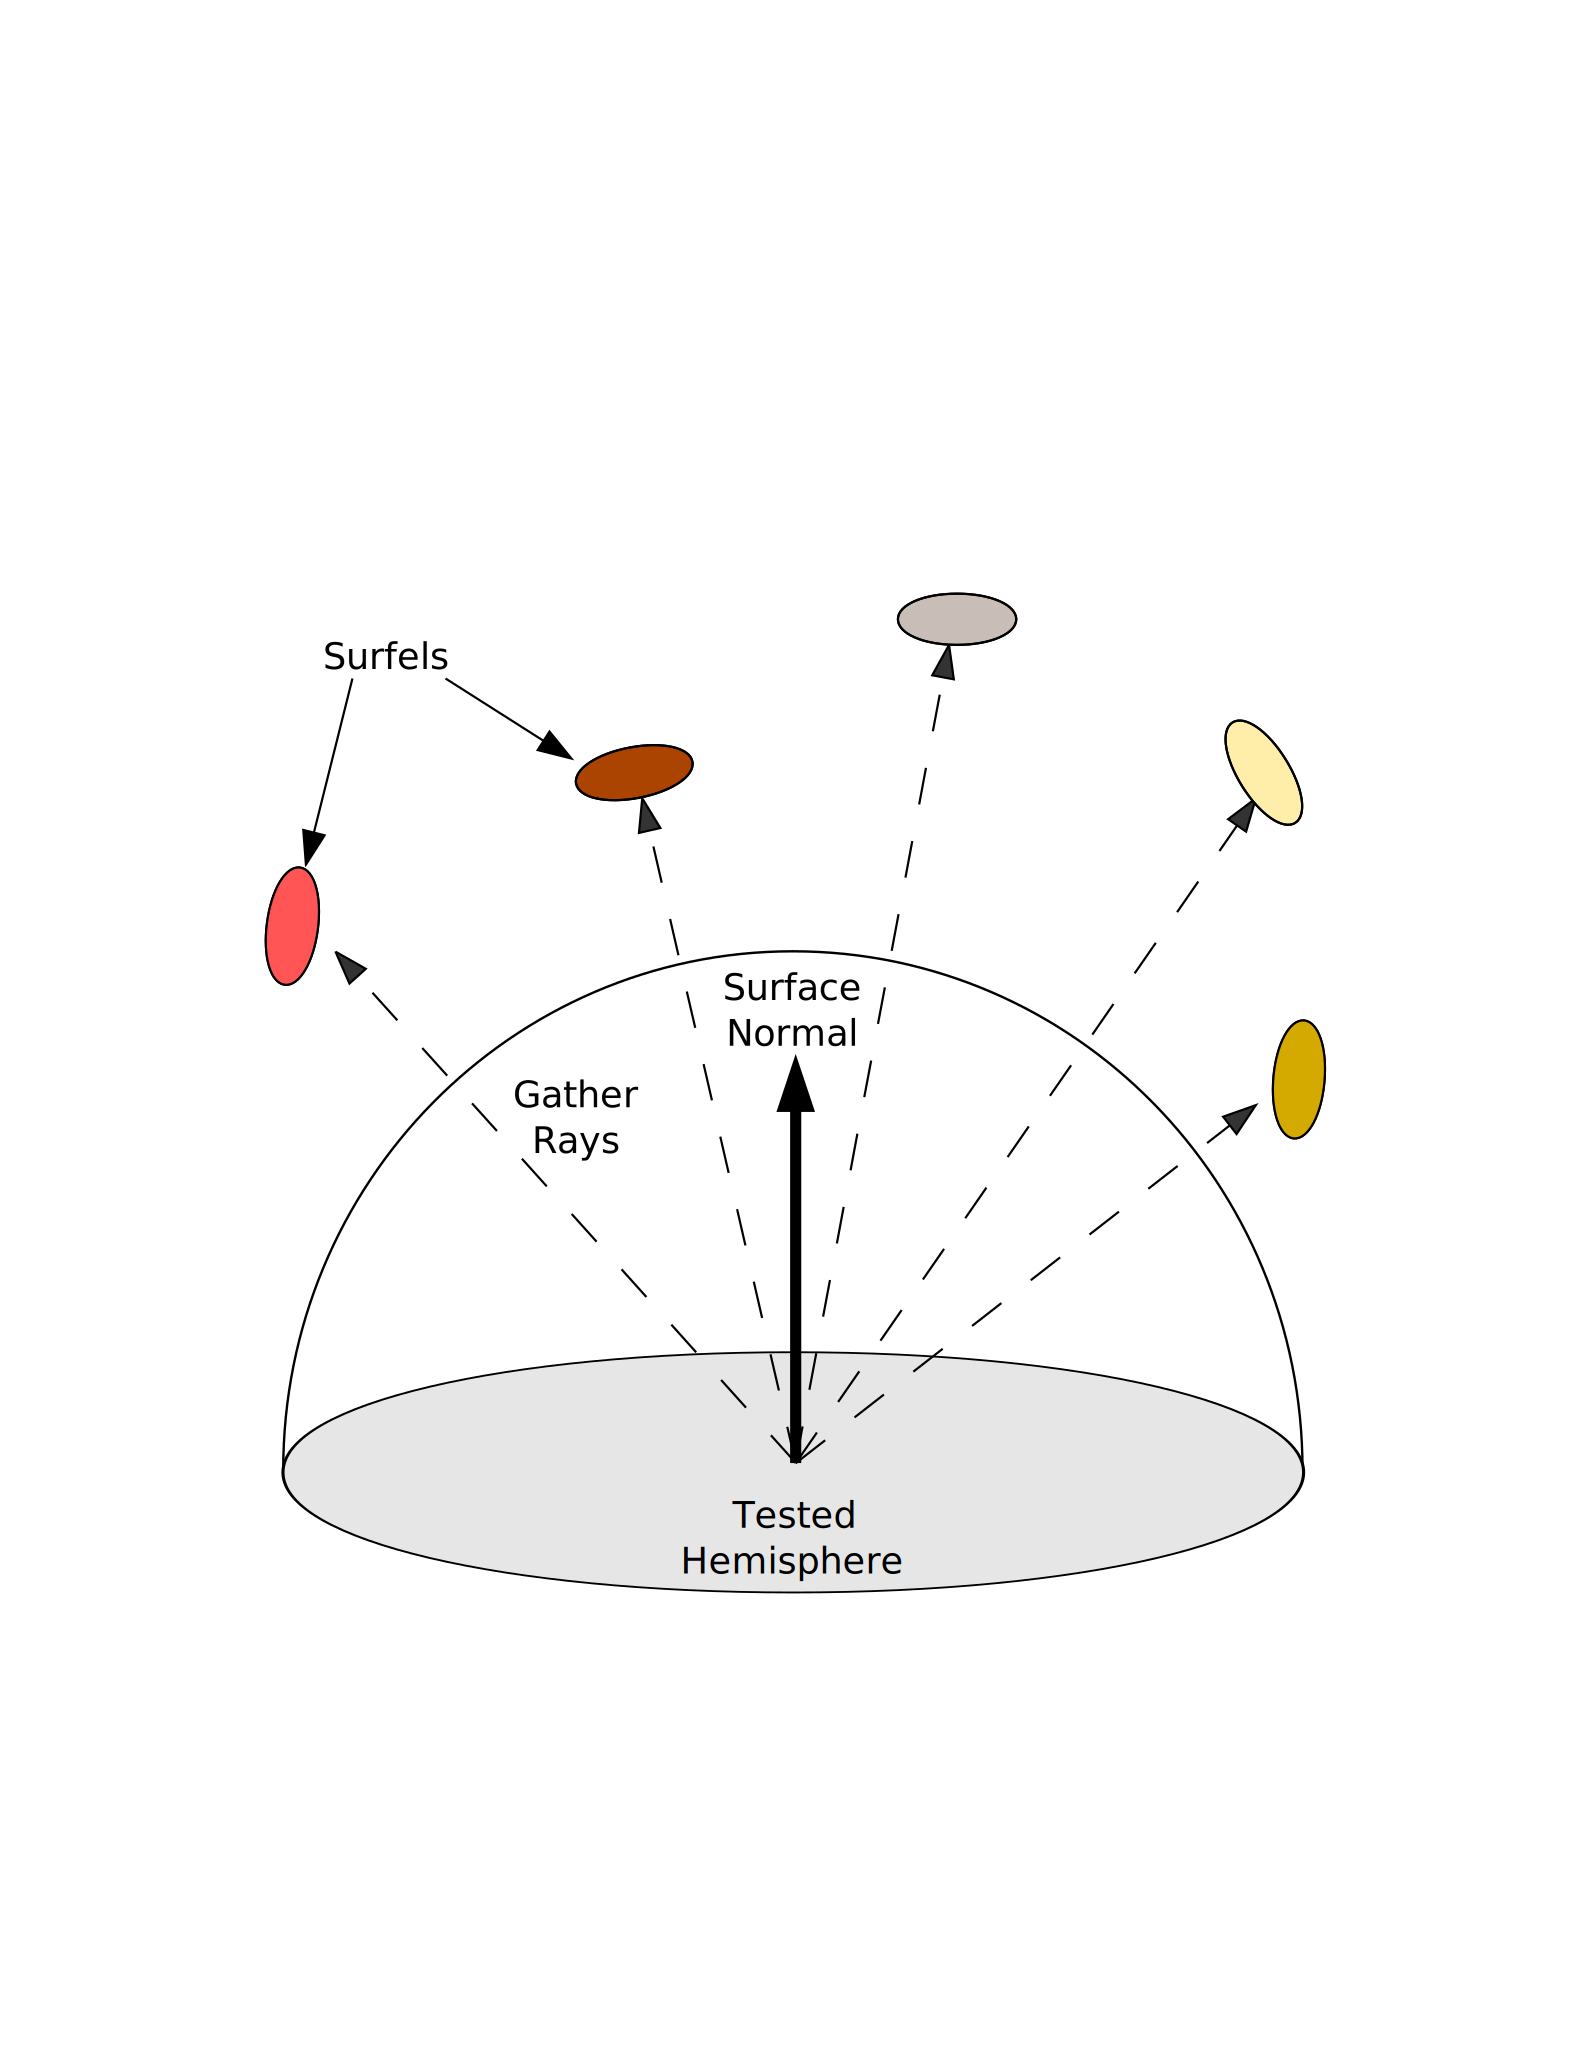
\includegraphics[height=\textwidth]{../img/diag/gather.pdf}\\
            \vspace{-4mm}
        \end{column}
    \end{columns}

    \centering
    

\end{frame}




\subsection{Integrating Volume Data}
%%--------------------------------------------------------------  PCB EXTENSION
\begin{frame}{Integrating Volume Data}

    \centering
    \includegraphics[height=70mm]{../img/testing.png}

\end{frame}




\section{Results}
%%--------------------------------------------------------------------  RESULTS
\begin{frame}{Results}

    \begin{center}
    \setlength{\tabcolsep}{5pt}
    \begin{tabular}{ | l | c | c | c | }
      \hline                       
      Scene & Render Time (s) & Image Delta & Memory Overhead \\
      \hline                  
      Monte Carlo w/o PCB & 3351 sec & NONE & NONE \\
      Traditional PCB & 348 sec & 11.0\% & 390 Mb (4.0\%) \\
      Extended PCB & 397 sec & 4.8\% & 395 Mb (4.1\%)  \\
      \hline  
    \end{tabular}
    \end{center}

\end{frame}




\section{Future Work}
%%--------------------------------------------------------------------  RESULTS
\begin{frame}{Future Work}

    \begin{enumerate}
        \item Multiple bounce
        \item Phase functions for volumes
        \item Parallelism
        \item Optimal Sampling
        \item GPU Acceleration
    \end{enumerate}

\end{frame}




\section{Conclusion}
%%-----------------------------------------------------------------  CONCLUSION
\begin{frame}{Conclusion}

    Oh yea!

\end{frame}

\end{document}
